\chapter{Flow Diagram}

\section{Overall System Flow}
\begin{figure}[H]
\centering
\begin{tikzpicture}[
    block/.style={draw, rounded corners, minimum width=3.5cm, minimum height=0.8cm, align=center, font=\footnotesize},
    arrow/.style={->, thick},
    node distance=1.2cm
]
\node[block, fill=green!20] (sensor) {IoT Sensors / Simulator};
\node[block, fill=blue!20, below of=sensor] (api) {POST /api/health-data};
\node[block, fill=red!20, below of=api] (alert) {Alert Checker\\(Threshold Evaluation)};
\node[block, fill=orange!20, below left=1cm and 0.5cm of alert] (db) {MongoDB\\(Store Data + Alerts)};
\node[block, fill=purple!20, below right=1cm and 0.5cm of alert] (socket) {Socket.IO\\(Broadcast Events)};
\node[block, fill=cyan!20, below=2.5cm of alert] (dashboard) {React Dashboard\\(Real-time Update)};

\draw[arrow] (sensor) -- (api);
\draw[arrow] (api) -- (alert);
\draw[arrow] (alert) -- (db);
\draw[arrow] (alert) -- (socket);
\draw[arrow] (socket) -- (dashboard);
\end{tikzpicture}
\caption{Data Pipeline Flow Diagram}
\label{fig:dataflow}
\end{figure}

\section{Authentication Flow}
\begin{figure}[H]
\centering
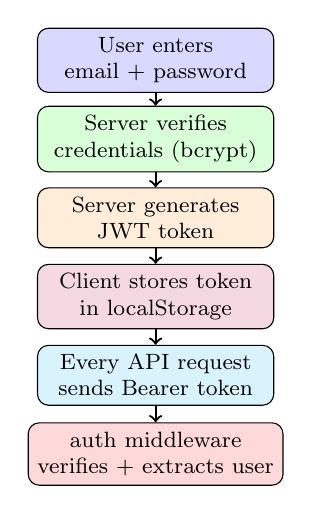
\begin{tikzpicture}[
    block/.style={draw, rounded corners, minimum width=3cm, minimum height=0.7cm, align=center, font=\footnotesize},
    arrow/.style={->, thick},
    node distance=1cm
]
\node[block, fill=blue!15] (login) {User enters\\email + password};
\node[block, fill=green!15, below of=login] (verify) {Server verifies\\credentials (bcrypt)};
\node[block, fill=orange!15, below of=verify] (jwt) {Server generates\\JWT token};
\node[block, fill=purple!15, below of=jwt] (store) {Client stores token\\in localStorage};
\node[block, fill=cyan!15, below of=store] (request) {Every API request\\sends Bearer token};
\node[block, fill=red!15, below of=request] (middleware) {auth middleware\\verifies + extracts user};

\draw[arrow] (login) -- (verify);
\draw[arrow] (verify) -- (jwt);
\draw[arrow] (jwt) -- (store);
\draw[arrow] (store) -- (request);
\draw[arrow] (request) -- (middleware);
\end{tikzpicture}
\caption{JWT Authentication Flow}
\label{fig:authflow}
\end{figure}

\section{Patient Registration \& Assignment Flow}
\begin{figure}[H]
\centering
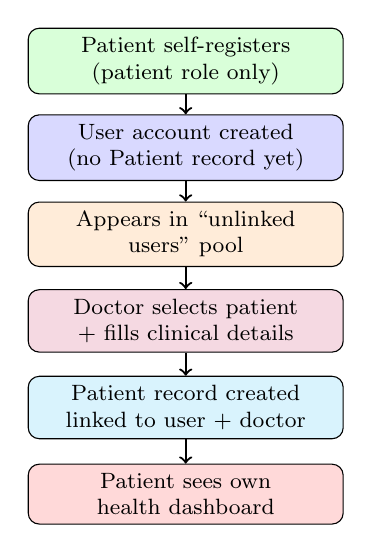
\begin{tikzpicture}[
    block/.style={draw, rounded corners, minimum width=4cm, minimum height=0.7cm, align=center, font=\footnotesize},
    arrow/.style={->, thick},
    node distance=1.1cm
]
\node[block, fill=green!15] (reg) {Patient self-registers\\(patient role only)};
\node[block, fill=blue!15, below of=reg] (account) {User account created\\(no Patient record yet)};
\node[block, fill=orange!15, below of=account] (pool) {Appears in ``unlinked\\users'' pool};
\node[block, fill=purple!15, below of=pool] (doctor) {Doctor selects patient\\+ fills clinical details};
\node[block, fill=cyan!15, below of=doctor] (linked) {Patient record created\\linked to user + doctor};
\node[block, fill=red!15, below of=linked] (access) {Patient sees own\\health dashboard};

\draw[arrow] (reg) -- (account);
\draw[arrow] (account) -- (pool);
\draw[arrow] (pool) -- (doctor);
\draw[arrow] (doctor) -- (linked);
\draw[arrow] (linked) -- (access);
\end{tikzpicture}
\caption{Patient Registration and Assignment Workflow}
\label{fig:patientflow}
\end{figure}

\section{Hardware Data Flow}
\begin{figure}[H]
\centering
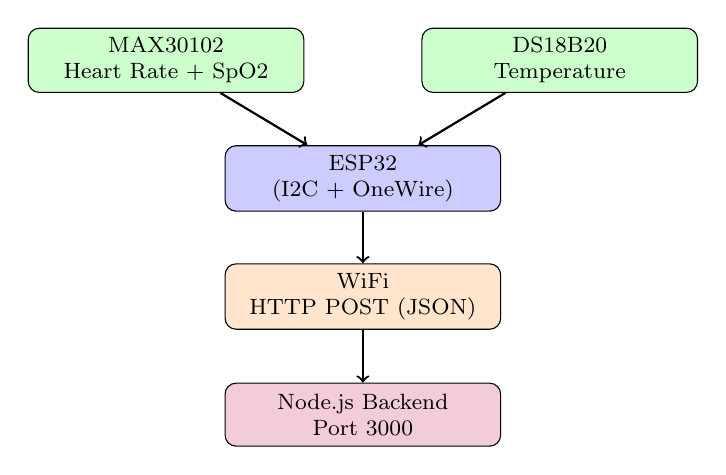
\begin{tikzpicture}[
    block/.style={draw, rounded corners, minimum width=3.5cm, minimum height=0.8cm, align=center, font=\footnotesize},
    arrow/.style={->, thick}
]
\node[block, fill=green!20] (max) at (0,3) {MAX30102\\Heart Rate + SpO2};
\node[block, fill=green!20] (ds) at (5,3) {DS18B20\\Temperature};
\node[block, fill=blue!20] (esp) at (2.5,1.5) {ESP32\\(I2C + OneWire)};
\node[block, fill=orange!20] (wifi) at (2.5,0) {WiFi\\HTTP POST (JSON)};
\node[block, fill=purple!20] (server) at (2.5,-1.5) {Node.js Backend\\Port 3000};

\draw[arrow] (max) -- (esp);
\draw[arrow] (ds) -- (esp);
\draw[arrow] (esp) -- (wifi);
\draw[arrow] (wifi) -- (server);
\end{tikzpicture}
\caption{Hardware Sensor Data Flow}
\label{fig:hwflow}
\end{figure}
